\documentclass[notheorems,mathserif,table,compress,dvipsnames]{beamer}  %dvipdfm选项是关键,否则编译统统通不过
%%------------------------常用宏包------------------------
%%注意, beamer 会默认使用下列宏包: amsthm, graphicx, hyperref, color, xcolor, 等等
\usepackage{fontspec,xunicode,xltxtra}  % for XeTeX
\usepackage{verbatim}
\usepackage{mathabx}
\usepackage{amsfonts,amssymb}
\usepackage{iplouclistings}
\usepackage{color}
\usepackage{fancybox}
%%------------------------ThemeColorFont------------------------
%% Presentation Themes
% \usetheme[<options>]{<name list>}
\usetheme{Madrid}
%% Inner Themes双精度计算
% \useinnertheme[<options>]{<name>}
%% Outer Themes
% \useoutertheme[<options>]{<name>}
\useoutertheme{miniframes} 
%% Color Themes 
%\usecolortheme[<options>]{<name list>}
%% Font Themes
\usefonttheme{serif}
\setbeamertemplate{background canvas}[vertical shading][bottom=white,top=structure.fg!7] %%背景色, 上25%的蓝, 过渡到下白.
\setbeamertemplate{theorems}[numbered]
\setbeamertemplate{navigation symbols}{}   %% 去掉页面下方默认的导航条.
\usepackage{zhfontcfg}
%\setsansfont[Mapping=tex-text]{文泉驿正黑}  %% 需要fontspec宏包
     %如果装了Adobe Acrobat,可在font.conf中配置Adobe字体的路径以使用其中文字体
     %也可直接使用系统中的中文字体如SimSun,SimHei,微软雅黑 等
     %原来beamer用的字体是sans family;注意Mapping的大小写,不能写错
     %设置字体时也可以直接用字体名,以下三种方式等同:
     %\setromanfont[BoldFont={黑体}]{宋体}
     %\setromanfont[BoldFont={SimHei}]{SimSun}
     %\setromanfont[BoldFont={"[simhei.ttf]"}]{"[simsun.ttc]"}
%%------------------------MISC------------------------
\graphicspath{{figures/}}         %% 图片路径. 本文的图片都放在这个文件夹里了.
%%------------------------正文------------------------
\begin{document}
\XeTeXlinebreaklocale "zh"         % 表示用中文的断行
\XeTeXlinebreakskip = 0pt plus 1pt % 多一点调整的空间
%%----------------------------------------------------------
%% This is only inserted into the PDF information catalog. Can be left
%% out.
%%%
%% Delete this, if you do not want the table of contents to pop up at
%% the beginning of each subsection:
%\AtBeginSection[]{                              % 在每个Section前都会加入的Frame
%  \frame<handout:0>{
%    \frametitle{Contents}\small
%    \tableofcontents[current,currentsubsection]
%  }
%}

%\AtBeginSubsection[]                            % 在每个子段落之前
%{
%  \frame<handout:0>                             % handout:0 表示只在手稿中出现
%  {
%    \frametitle{Contents}\small
%    \tableofcontents[current,currentsubsection] % 显示在目录中加亮的当前章节
%  }
%}
%
%%----------------------------------------------------------
\title{Partial Differential Equation and Image Processing}
\subtitle{~~~~~-An introduction to the BibDesk and Week Summary}
\author[Qiu]{\textcolor{olive}{QiuXinxin}}
\institute[OUC]{\small\textcolor{violet}{Ocean University of China}\\
\small\textcolor{violet}{College of Information Science and Engineering}}
\date{August 29, 2014}
%\titlegraphic{\vspace{-6em}\includegraphics[height=7cm]{ouc}\vspace{-6em}}
\frame{ \titlepage }
%%----------------------------------------------------------
\section*{Contents}
\frame{\frametitle{}\tableofcontents}
%%----------------------------------------------------------
\section{An introduction to BibDesk}
%
\begin{frame}
\frametitle{BibDesk}
\begin{itemize}
\item 
BibDesk is an open-source reference management software package for Mac OS X, used to manage bibliographies and references when writing essays and articles.
\item BibDesk offers a front-end for creating, editing, managing, and searching BibTeX databases.
\item BibDesk's services will simplify using your bibliography in other applications and are particularly well suited for \LaTeX  users.
\end{itemize}
\end{frame}

%
\begin{frame}
\frametitle{}
\begin{figure}[!ht]
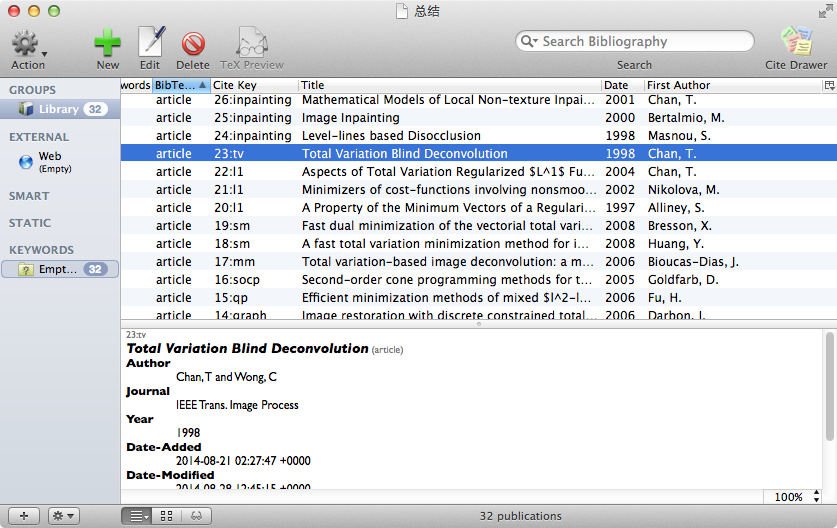
\includegraphics[width=4.2in]{bibdesk1}
\caption{Screen shot of BibDesk (Version 1.6.3)}
\end{figure} 
\end{frame}

%
\begin{frame}
\frametitle{How to use the BibDesk}
\begin{figure}[!ht]
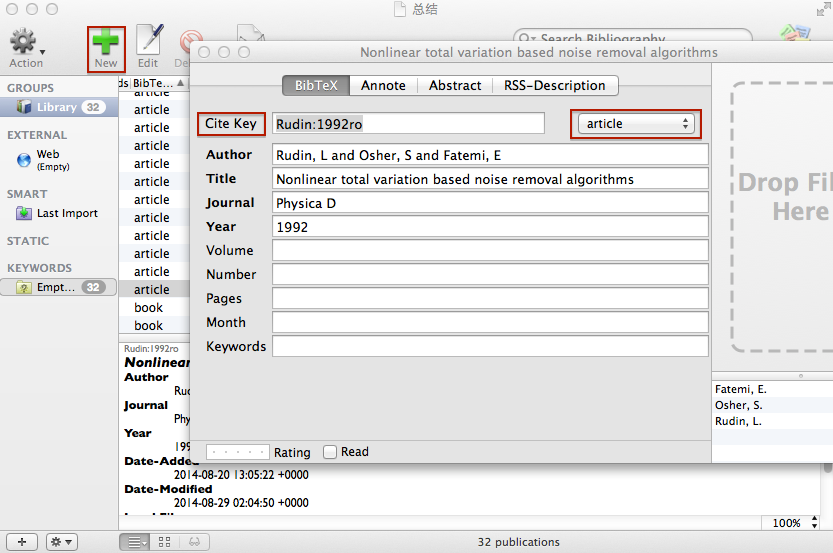
\includegraphics[width=4.2in]{bibdesk2}
\end{figure} 
\end{frame}

%
\begin{frame}
\frametitle{Publication Editor}
\begin{figure}[!ht]
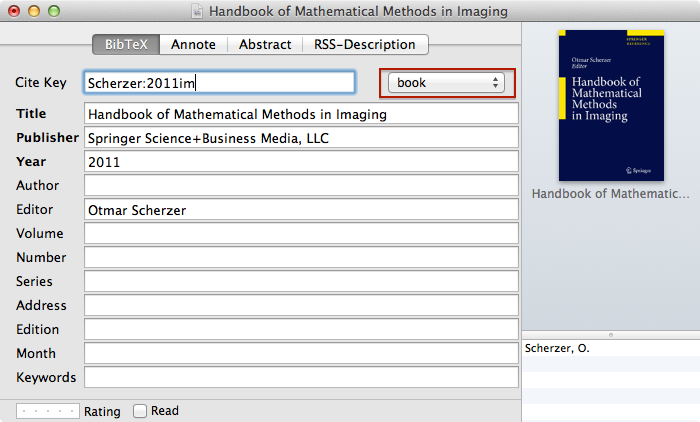
\includegraphics[width=4.2in]{bibdesk3}
\end{figure} 
\end{frame}

%
\begin{frame}
\frametitle{Cite Key}
\begin{figure}[!ht]
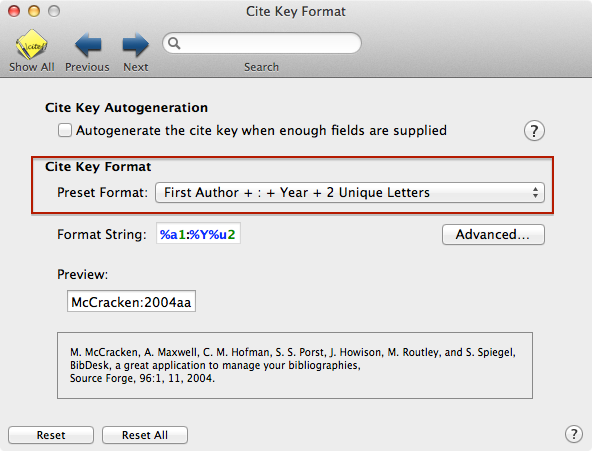
\includegraphics[width=3.7in]{bibdesk7}
\end{figure} 
\end{frame}

%
\begin{frame}
\frametitle{Notice}
\begin{itemize}
\item Formatting Names: Author and editor lists in BibTeX files are written as a single string using the word ``and" as a separator between names, like this example:
\begin{displaymath}
\textrm{``Adam Maxwell and Michael O. McCracken"}
\end{displaymath}

\item If a name has two parts, commas are used to determine which parts are the first, middle and last names. For example, the following two names are the same: 
\begin{displaymath}
\textrm{``Adam Maxwell" and ``Maxwell, Adam"}
\end{displaymath}
 
\end{itemize}
\end{frame}


%
\begin{frame}
\frametitle{Web search}
\begin{figure}[!ht]
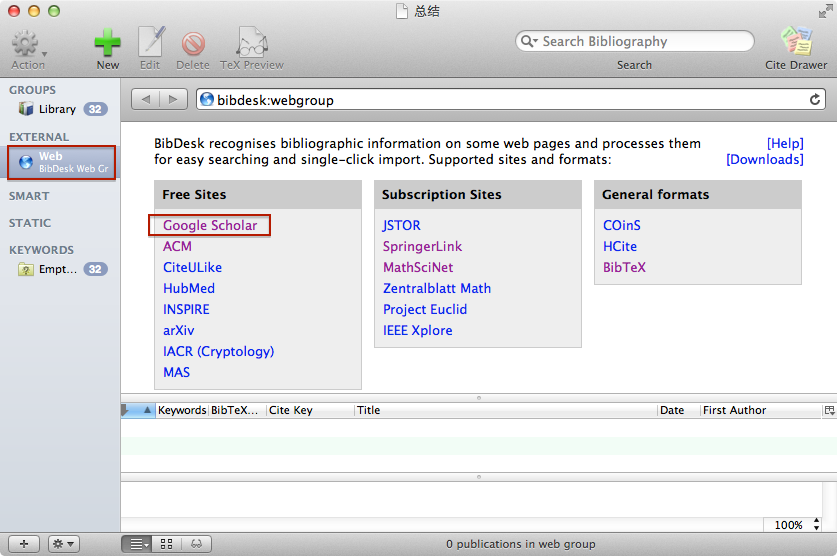
\includegraphics[width=4.2in]{bibdesk4}
\end{figure} 
\end{frame}


%
\begin{frame}
\frametitle{Web search}
\begin{figure}[!ht]
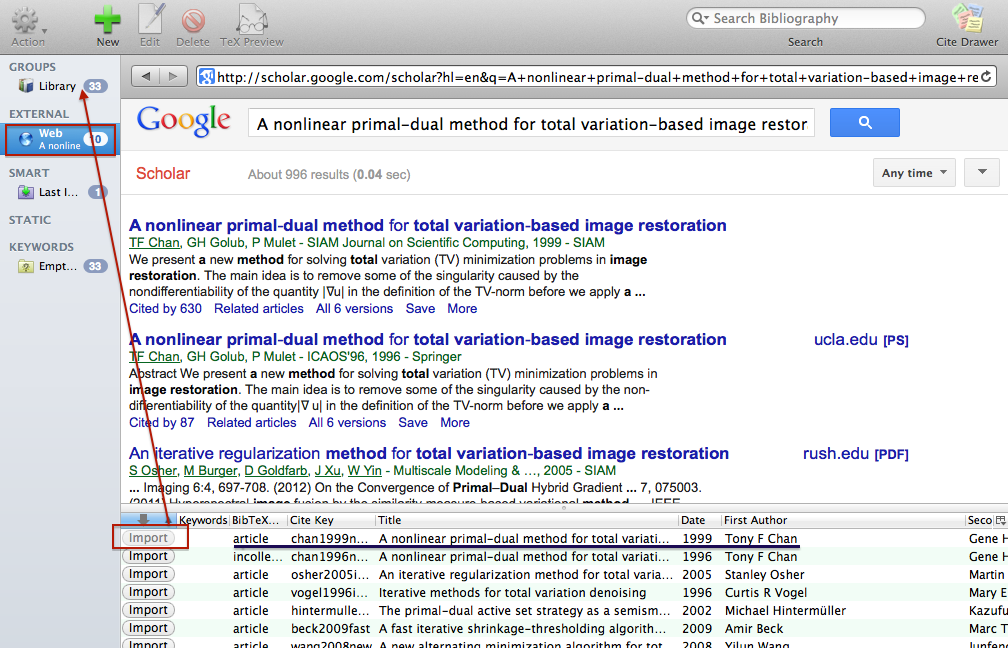
\includegraphics[width=4.2in]{bibdesk5}
\end{figure} 
\end{frame}

%
\begin{frame}
\frametitle{Web search}
\begin{figure}[!ht]
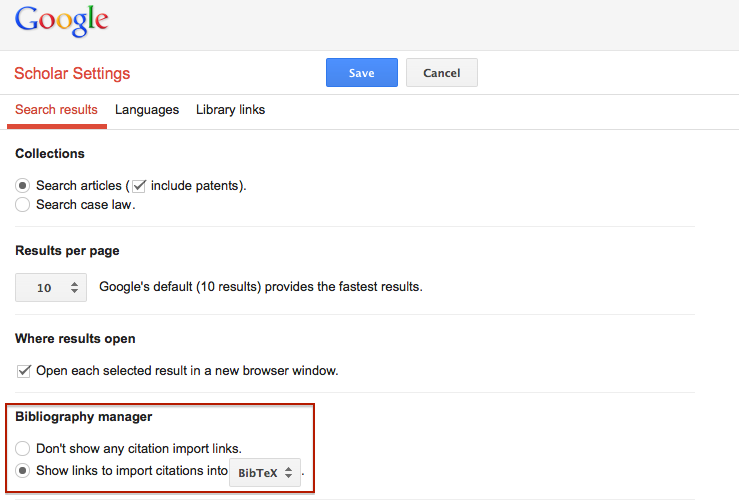
\includegraphics[width=4.2in]{bibdesk8}
\end{figure} 
\end{frame}

%
\begin{frame}
\frametitle{}
\begin{enumerate}
\item Export the file as BibTex format
\item Run the tex-file once
\item Run the bib-file once
\item Run the tex-file twice 
\end{enumerate}
\begin{itemize}
\item The cite key of bib-file must be consistent with the citation-name of tex-file
\item More information can be found in the website \url{http://bibdesk.sourceforge.net/}
\end{itemize}
\end{frame}

%
\begin{frame}
\frametitle{Export BibTex}
\begin{figure}[!ht]
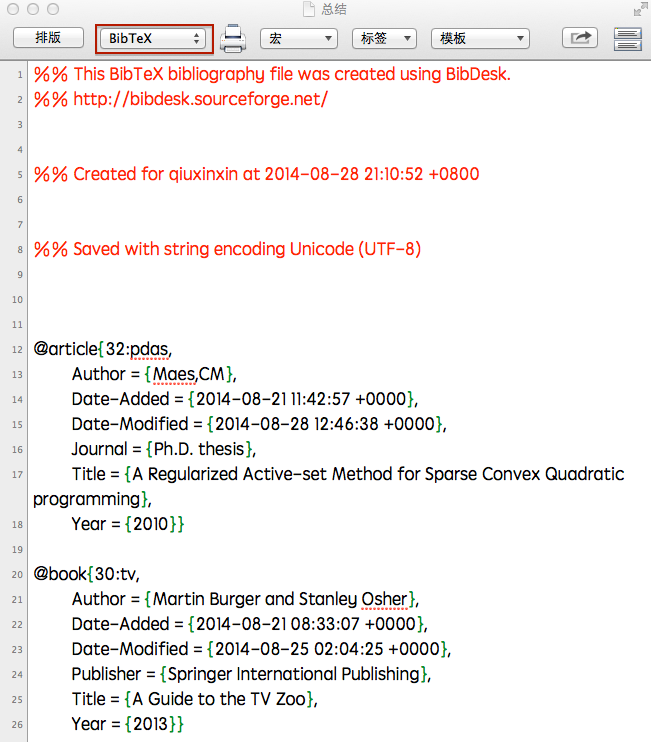
\includegraphics[width=2.5in]{bibdesk6}
\end{figure} 
\end{frame}

\section{Week summary}

%
\begin{frame}
\frametitle{Week summary}
\begin{itemize}
\item Reading the matlab code of the paper
\item Searching and organize the papers
\end{itemize}
\end{frame}

\end{document}
